\begin{figure}
\centering
\begin{tikzpicture}
  \node[inner sep=0pt] (circuit) at (0,0) {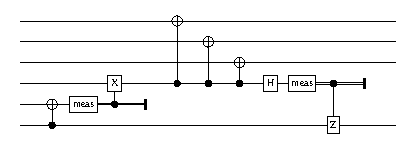
\includegraphics[scale=2]{Figures/circuits/nonlocalCNOTs}};
  \pic (e1) {ebit=e1/26.79mm/13mm};
  \pic [below left=27mm and -13mm of circuit.north west] (entangler) {box=entangler/23.5mm/52mm/23mm/38mm/Entangler/0mm/1mm};
  \pic [below left=27mm and -13mm of circuit.north west] (disentangler) {box=disentangler/23.5mm/126mm/23mm/38.5mm/Disentangler/10.5mm/1mm};
  \coordinate[below left=7mm and -6mm of circuit.west] (leftPoint);
  \coordinate[right=130.5mm of leftPoint] (rightPoint);
  \pic (cut) {cut=leftPoint/rightPoint};
\end{tikzpicture}
\caption{Implementing multiple non-local CNOTs using a single ebit. The bottom-most wire acts as control for the three of them. Only classical information crosses the boundary between QPUs.}
\label{fig:nonLocalCNOTs}
\end{figure}